\newpage

\section*{ Aluminium }

Power Level: 100 kW(th) \\
Time at Power: 3600 s \\
Wait Time: 354870 s \\
Total Activity at Removal: 8.36e+01 $\mu Ci$

\begin{table*}[h]
\centering
\begin{tabular}{ |c|c|c|c|c|c|c| }
 \hline
 Position & Mass $mg$ & Start Counting $s$ & Counting Time $s$ & Counting Activity $\mu Ci$ & Expected Area (Counts) \\
 \hline 
 1 & 0.3 & 358470 & 3600 & 6.27e-05 & -1.11e-21\\ 
\hline
 2 & 0.2 & 362070 & 3600 & 6.09e-05 & 1.28e-20\\ 
\hline
 3 & 0.1 & 365670 & 3600 & 2.25e-05 & -3.82e-21\\ 
\hline
 4 & 0.2 & 369270 & 3600 & 2.00e-05 & 1.40e-22\\ 
\hline
\end{tabular}
\end{table*}

\begin{figure}[!ht]
   \centering
   \subfloat[][Position \#1]{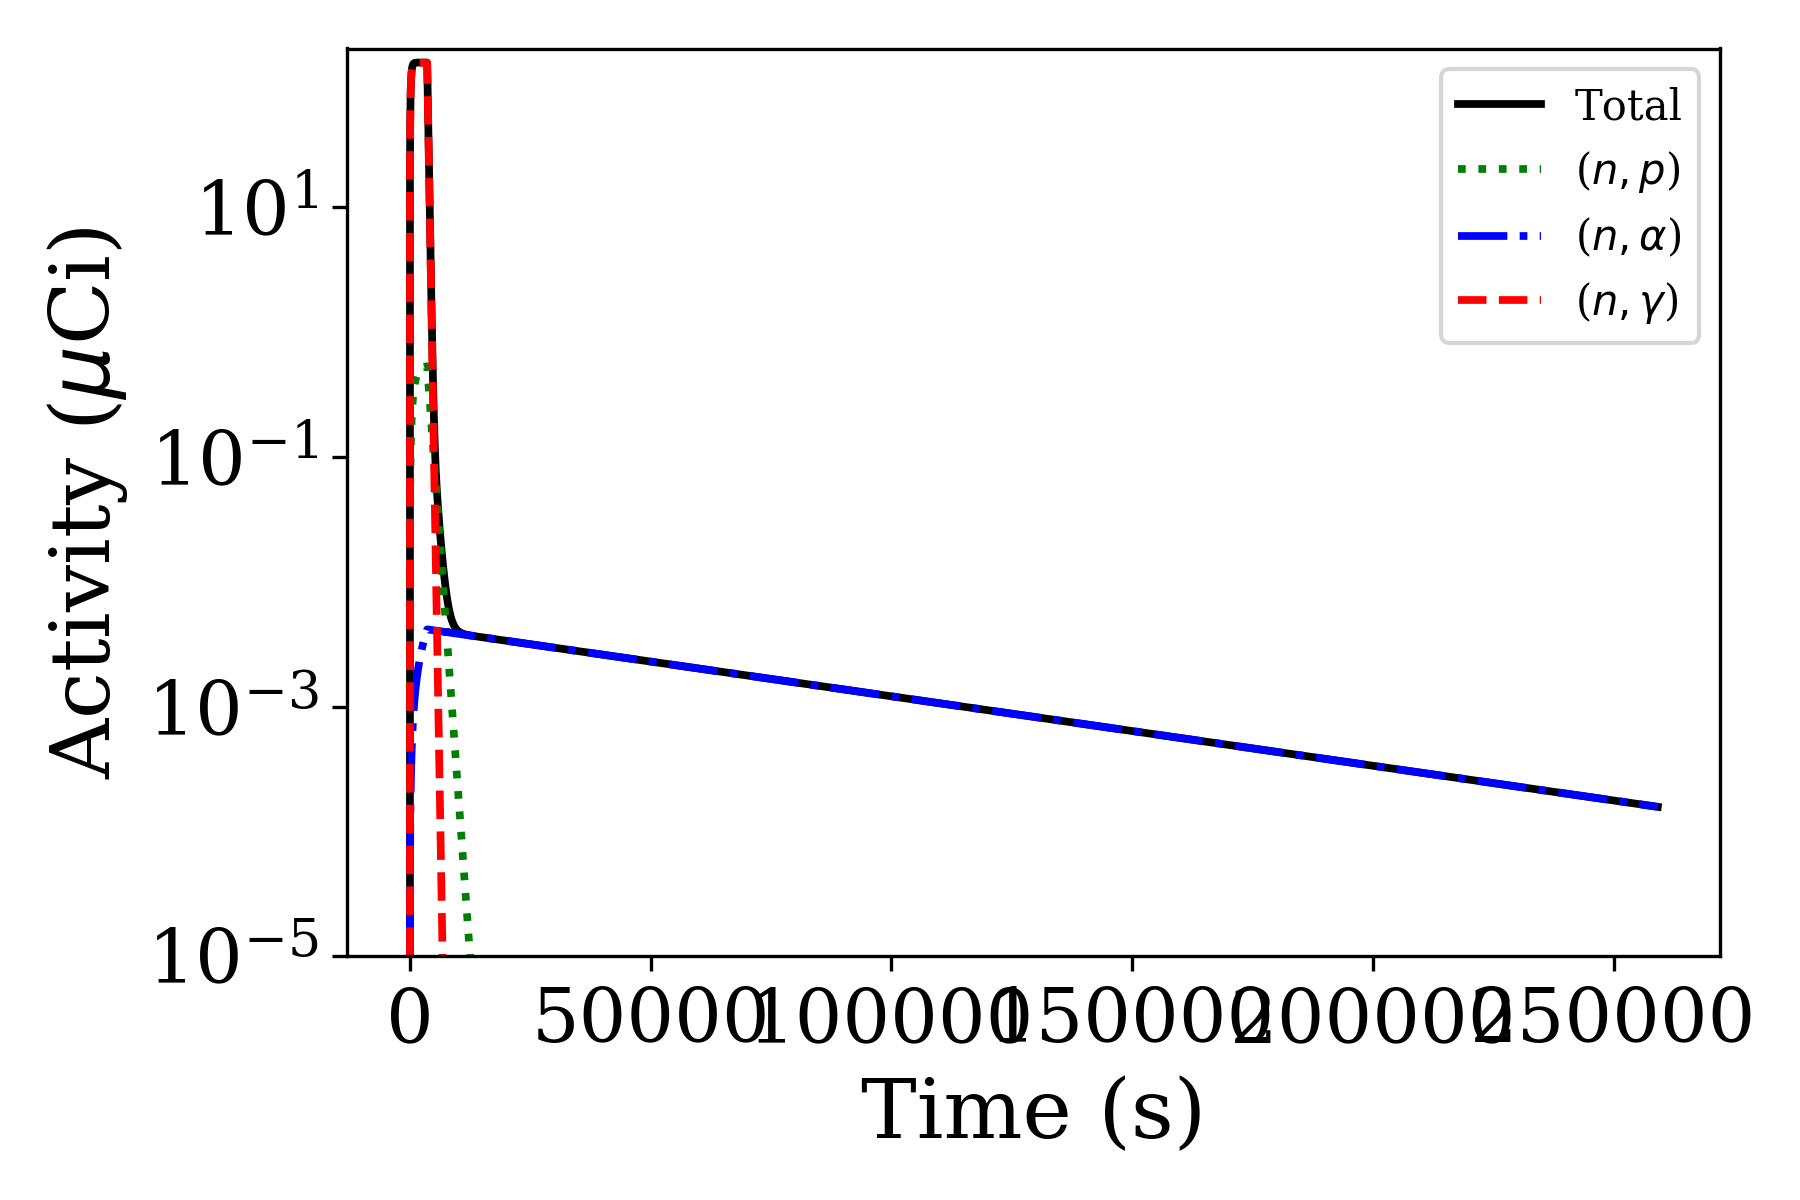
\includegraphics[width=.4\textwidth]{source/plot/al1_activity}}\quad
   \subfloat[][ ($n,p$) Reaction Rate]{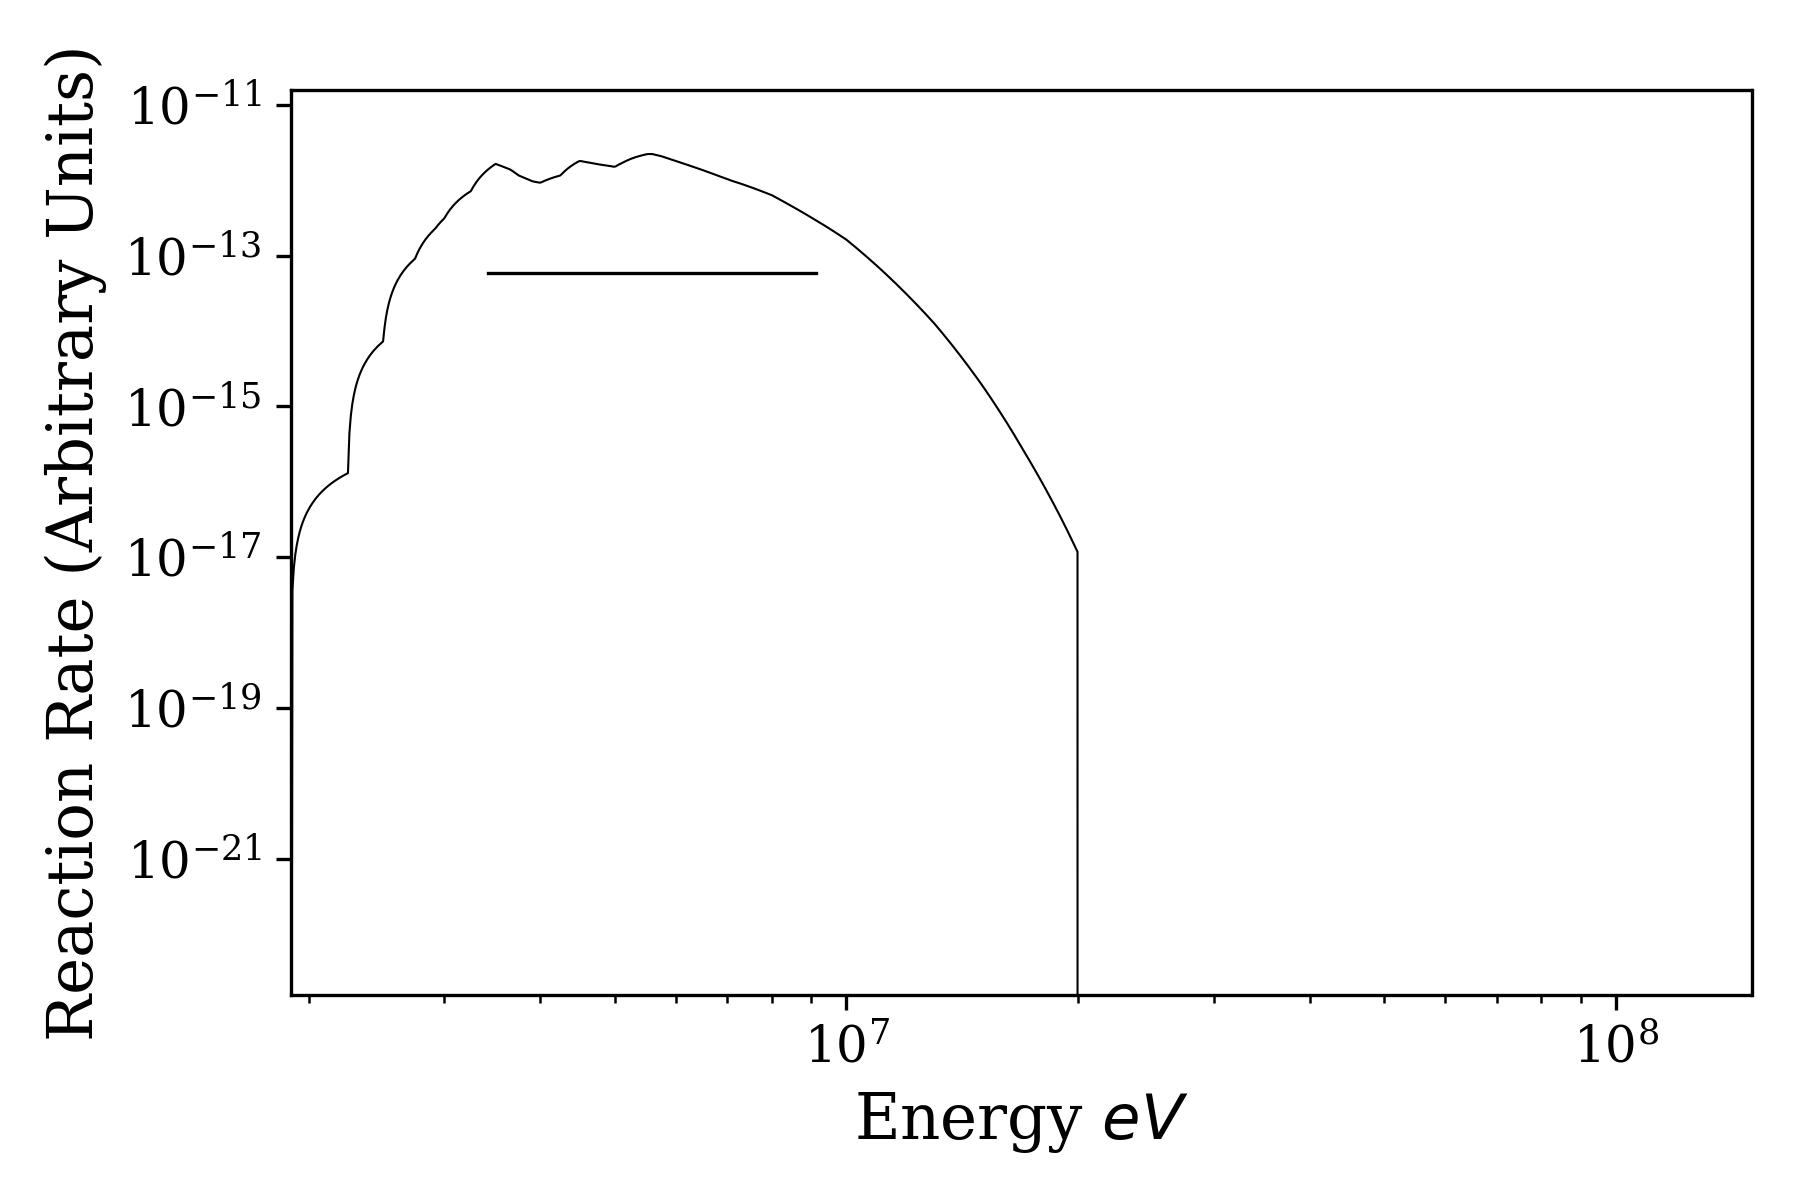
\includegraphics[width=.4\textwidth]{source/plot/al_n,p}}\\ 
   \subfloat[][ ($n,\alpha$) Reaction Rate]{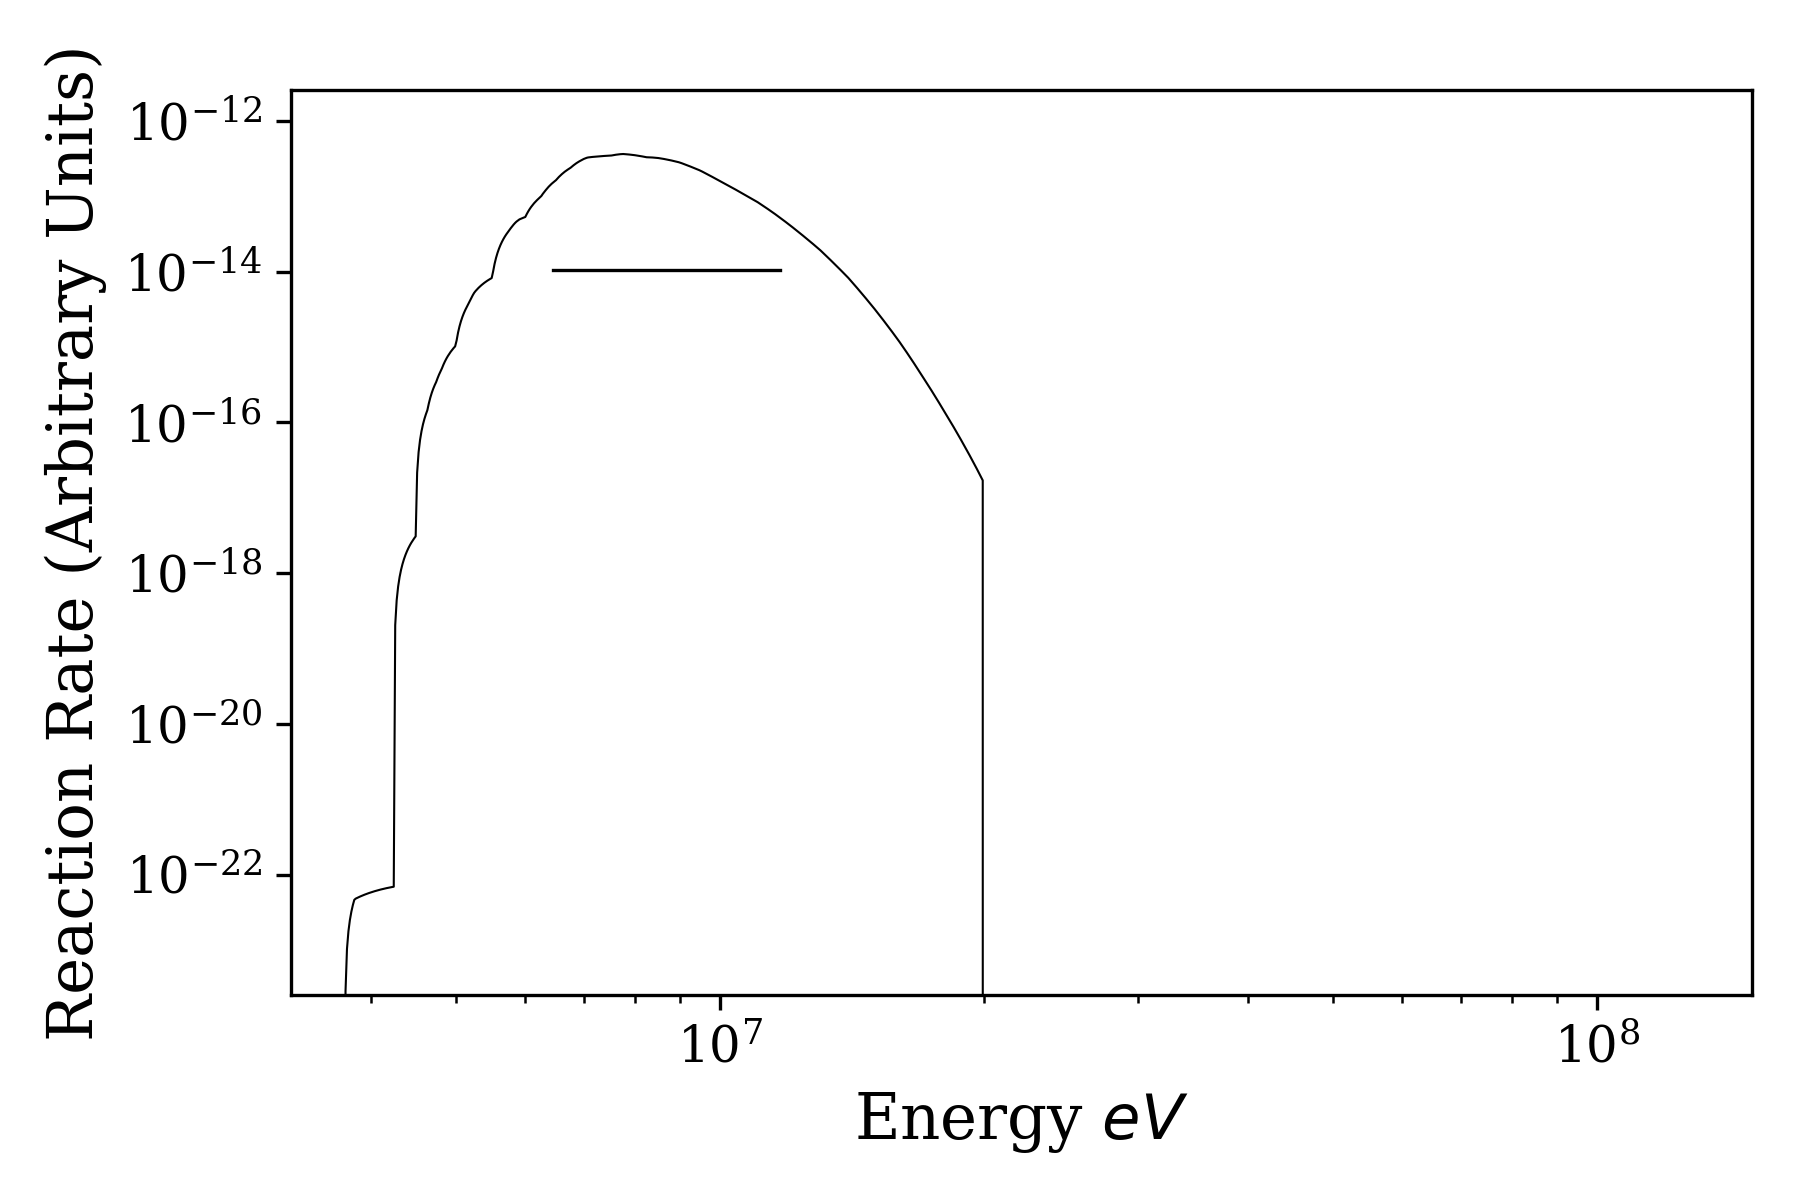
\includegraphics[width=.4\textwidth]{source/plot/al_n,alpha}}\quad 
   \subfloat[][ ($n,\gamma$) Reaction Rate]{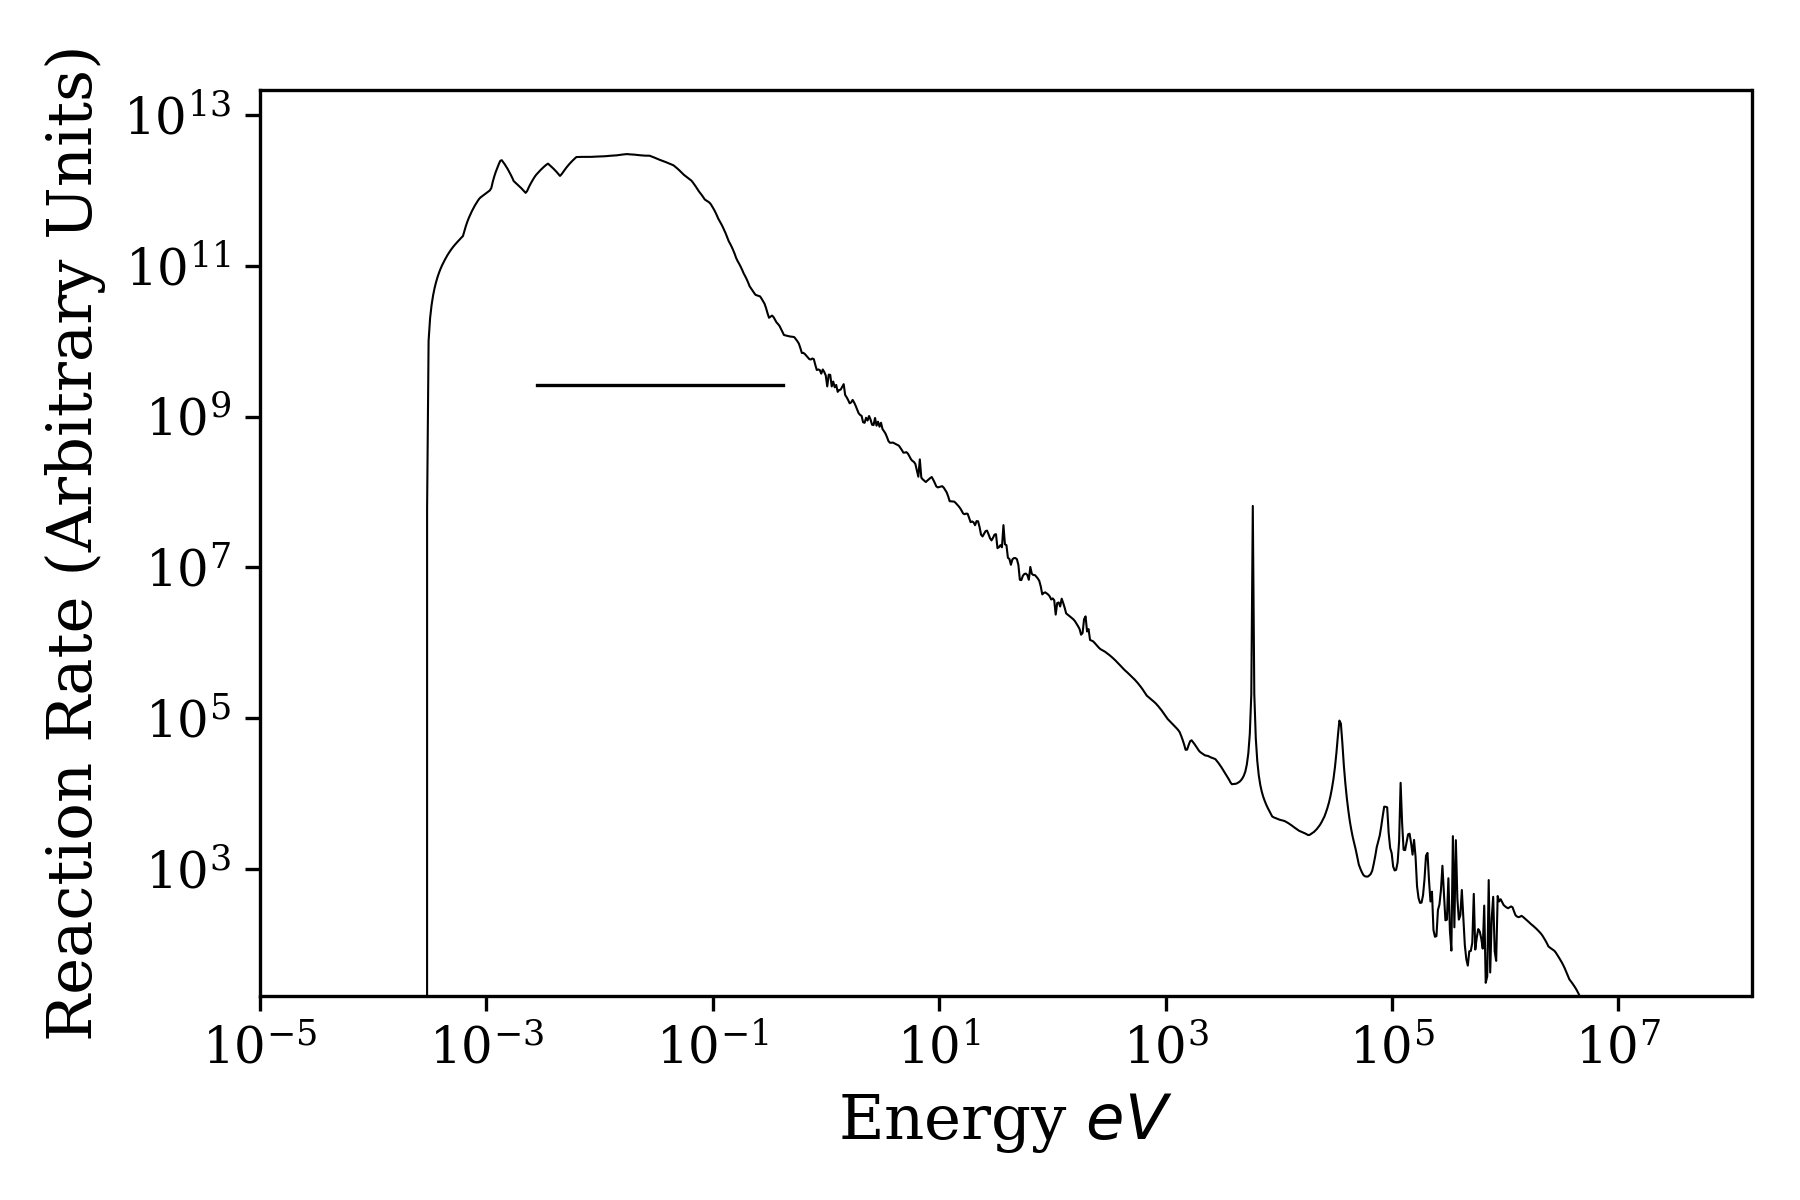
\includegraphics[width=.4\textwidth]{source/plot/al_n,gamma}}\\ 

\end{figure}

\begin{table*}[h]
\centering
\begin{tabular}{ |c|c|c|c|c|c|c| }
 \hline
 Reaction & T$_{1/2}$ & ROI (eV) & Important Gammas (keV) \\
 \hline 
 ($n,p$) &  9.5 m & 3.44e+06, 9.21e+06 & 180(0.007), 840(0.7), 1013(0.3) \\ 
\hline
 ($n,\alpha$) & 15.0 h & 6.48e+06, 1.07e+07 & 1369(1), 2754(1) \\ 
\hline
 ($n,\gamma$) &  2.2 m & 6.67e-03, 4.15e+00 & 1780(1) \\ 
\hline
\end{tabular}
\end{table*}
